\documentclass[10pt]{article}
\usepackage[polish]{babel}
\usepackage[utf8]{inputenc}
\usepackage[T1]{fontenc}
\usepackage{graphicx}
\usepackage[export]{adjustbox}
\graphicspath{ {./images/} }
\usepackage{amsmath}
\usepackage{amsfonts}
\usepackage{amssymb}
\usepackage[version=4]{mhchem}
\usepackage{stmaryrd}

\title{Zadania - etap II (szkoła podstawowa) }

\author{}
\date{}


\begin{document}
\maketitle
CENTRUM NAUCZANIA MATEMATYKI\\
I KSZTALCENIA NA ODLEGŁOSĆ

Zadanie 1. Suma czterech liczb wynosi 160 . Jakie to liczby, jeżeli pierwsza z nich jest mniejsza od drugiej o 10 , od trzeciej o 15 oraz jest dwa razy mniejsza od czwartej z nich?

Zadanie 2. Jeżeli pewną liczbę dwucyfrową podzielimy przez sumę jej cyfr, to otrzymamy 6 i resztę 3. Jeśli natomiast tę liczbę podzielimy przez sumę jej cyfr powiększoną o 2 , to otrzymamy 5 i resztę 5 . Co to za liczba?

Zadanie 3. Kwadrat o boku 15 cm podzielono linią prostą (patrz rysunek) tak, że powstały dwa trapezy, których obwody różniły się o 12 cm . Oblicz pola każdego z otrzymanych trapezów.\\
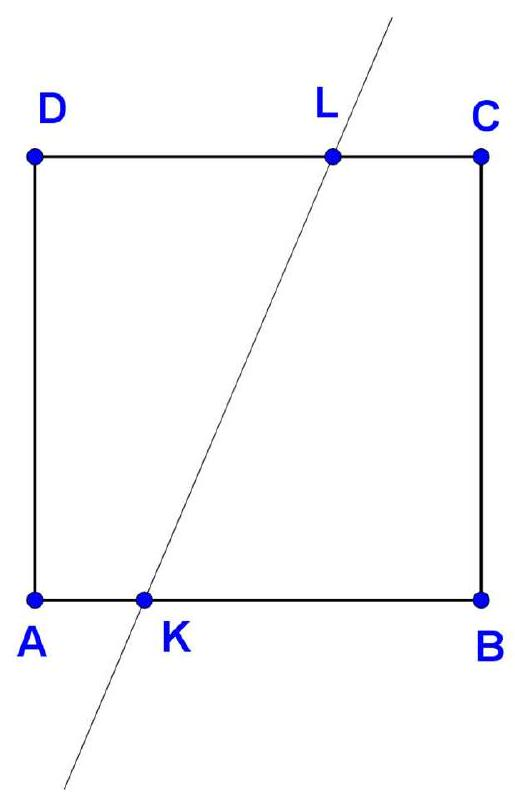
\includegraphics[max width=\textwidth, center]{2024_11_21_37063edf61ec0399ce4dg-1}

Zadanie 4. Udowodnij, że liczba: \(2^{59}+2^{60}+2^{61}\) dzieli się przez 14.\\
Zadanie 5. Z miast \(A\) i \(B\), odległych o 140 km , wyjechali o tym samym czasie na spotkanie dwaj rowerzyści, z których jeden jechał z prędkością \(15 \mathrm{~km} / \mathrm{h}\) a drugi z prędkością \(20 \mathrm{~km} / \mathrm{h}\) Po ilu godzinach jazdy się spotkali? Ile kilometrów przejechał każdy z nich?


\end{document}